\prologue{The sheer volumne of answers can often stifle insight...The purpose
of computing\index{computing!the purpose} is insight, not numbers.}
{Hamming}

\section{Definisi}
Sistem Informasi Geografis merupakan penggalan kata dan Sistem Informasi dan Geografis. Geografis dipandang sebagai bentukan dari geospasial.
Geospasial memiliki arti geo yang berarti bumi dan spasial yang berarti ruang atau keruangan. Jadi geospasial merupakan ilmu yang mempelajari 
tata ruang dari bumi. Tata ruang melingkupi letak suatu titik di bumi baik itu letak kota, provinsi atau negara. Tata ruang juga menyajikan gambaran dari ruang tersebut yang disebut dengan ilmu kartografi atau sering disebut sebagai ilmu pembuatan peta\cite{IEEEhowto:IEEEtranpage}.

\section{Sejarah Peta}
Perkembangan peta dunia tidak luput dari para ahli geografi dan kartografi. Peta dunia yang populer pada saat ini merupkan kontribusi dari para 
pembuat peta sebelumnya

\subsection{Ptolemy's}
Ptolemy's diduga membuat peta pada abad ke 2


\subsection{Muhammad al-Idrisi}
Seorang ahli geografi dan kartografi Muhammad al-Idrisi membuat peta dunia pada abad ke 11

\begin{figure}[ht]

\centerline{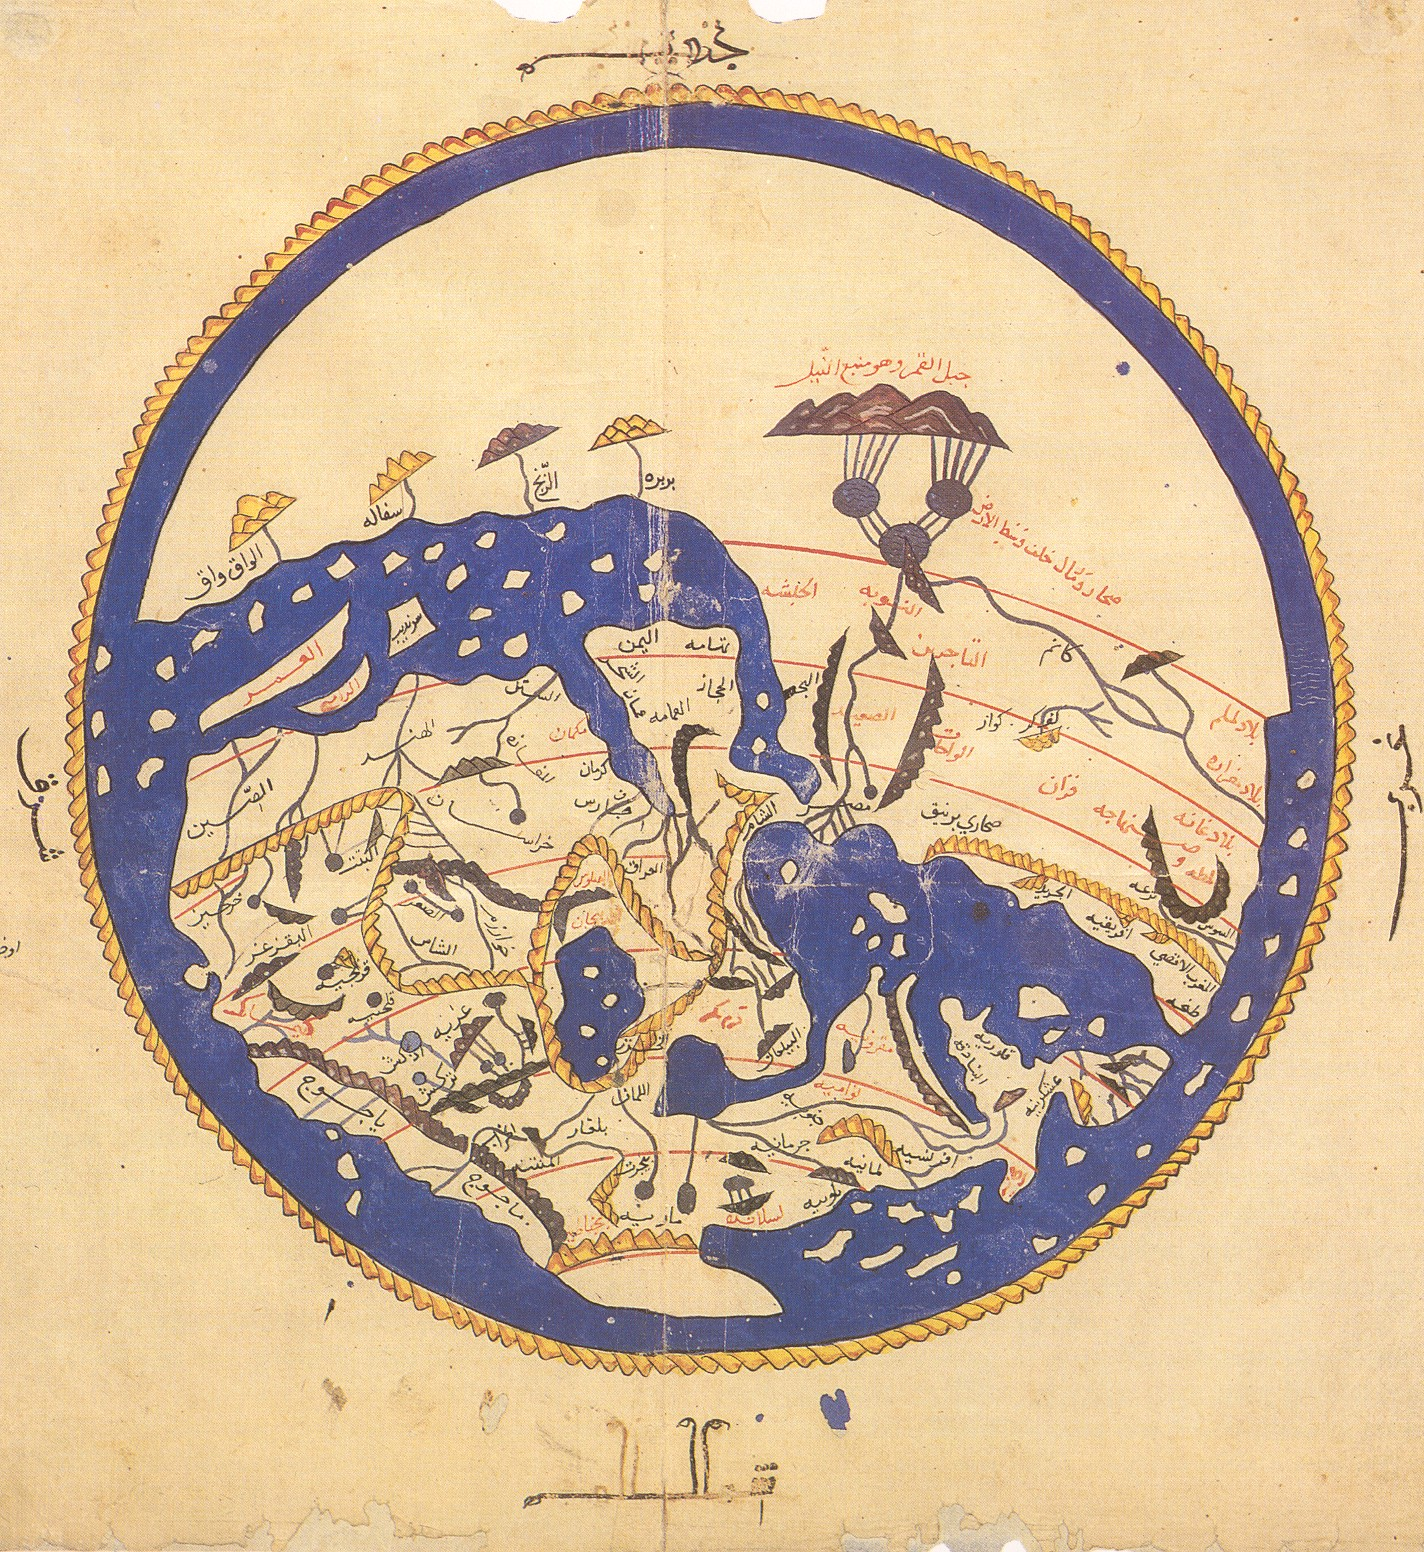
\includegraphics[width=1\textwidth]{figures/petaduniaalid.JPG}}
\caption{Gambaran pengantar peta dunia karya al-Idrisi tahun 1154.}
\end{figure}

\begin{figure}[ht]
	\centerline{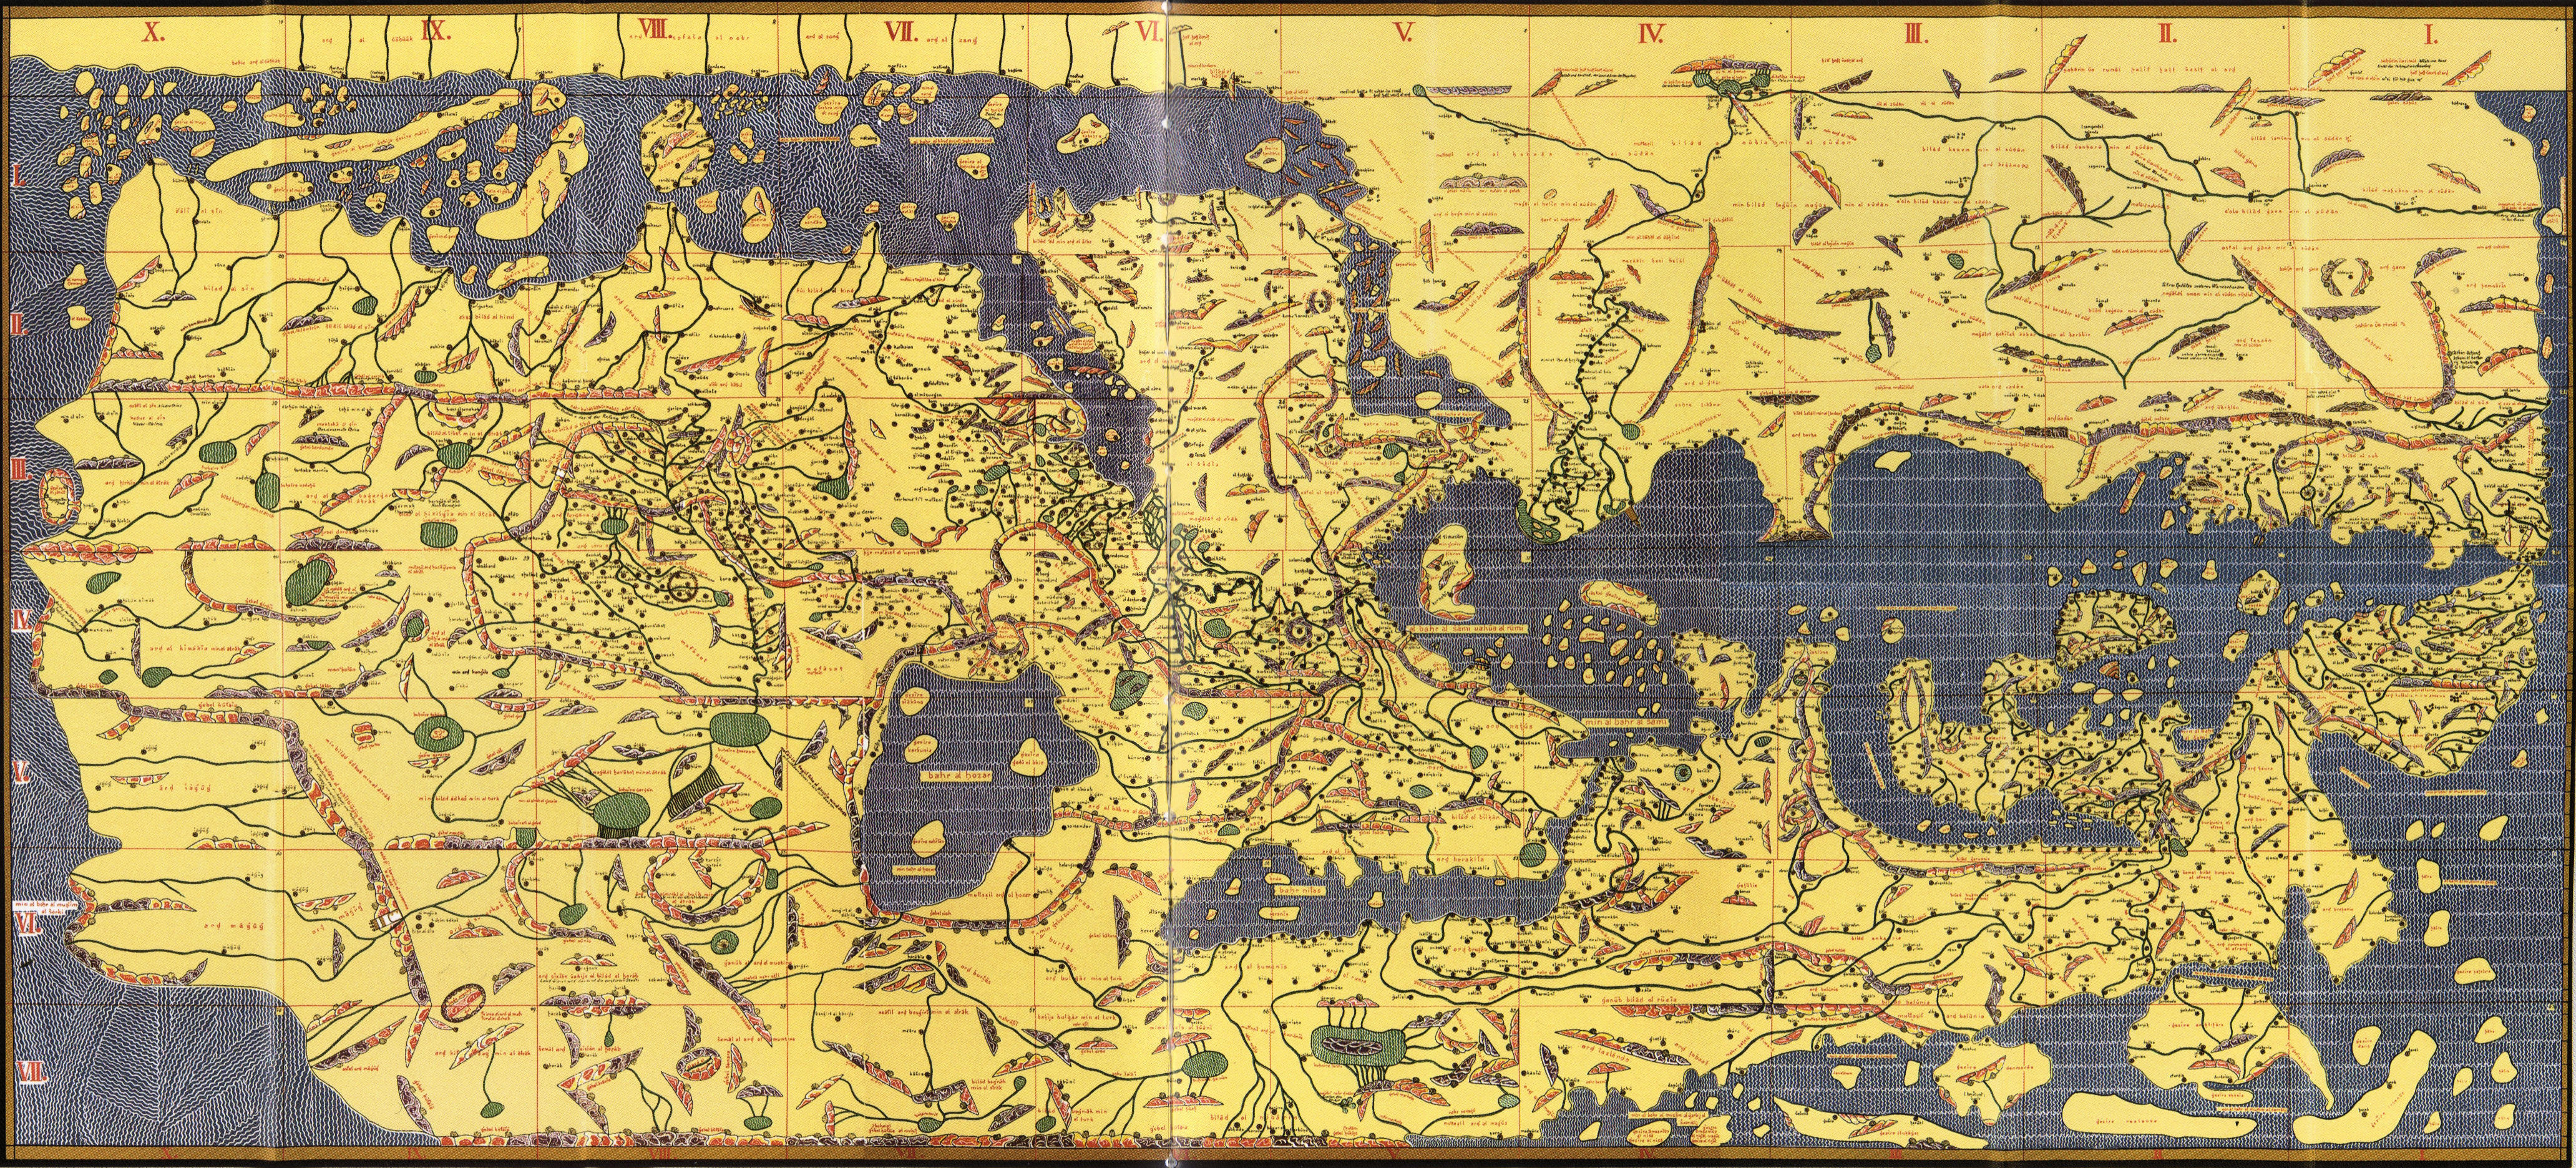
\includegraphics[width=1\textwidth]{figures/TabulaRogeriana.jpg}}
\vskip2pt
\caption{Tabula Rogeriana digambar oleh Al-Idrisi pada tahun 1154 untuk Raja Normandia Roger II dari Sisilia, setelah delapan menetap di istananya, di mana dia bekerja untuk penjelasan dan ilustrasi peta.}
\end{figure}

\section{Penentuan Kordinat}
Kordinat digunakan untuk mengacu sebuah titik lokasi di muka bumi, adapun beberapa jenis standar kordinat yang digunakan adalah.

\subsection{Kordinat Internasional}
Kordinat internasional dikenal dengan long dan lat.


\subsection{Kordinat Indonesia}
Masih ingatkah pelajaran geografi tentang letak Indonesia? maka kita bisa melihat jawaban tersebut dalam kordinat berbahasa indonesia.
